\newtheorem{problem}{Problem}[section]
%\newcommand{\inch}{\ensuremath{\,\textrm{in.}}}

\chapter{One-dimensional Steady State Problems}

\section{Overview}
This Chapter mainly discussed different kind of one-dimensional steady state problems. Including the use of Fourier’s law on constant cross sectional and non uniform cross sectional problem , the one dimensional steady state problem with constant and variate heat generation problem in both catesian and cylindrical coodinate system, and the fin design under steady state.

\section{Fourier's law}

\begin{example}
\label{example:2:1}
\textbf{Fourier’s law, plane wall, constant internal heat
generation.} \textcolor{blue} {\emph{Refer to tutorial Fourier’s
law.nb, and Ch. 2, P. 69.}} Consider a one-dimensional plane wall in steady state and without heat generation.
Temperature on one side is $T_0=50~K$, other side is $T_1=30~K$, wall width is $L=0.01~m$,
area is $A=1~m^2$, thermal conductivity $k=0.5~W/m.k$. Sketch the heat distribution on T-x coordinate,
what is the heat flux  through the wall? (As shown in figure \ref{fig:2:1})
\begin{figure}[h!]
  \centering
    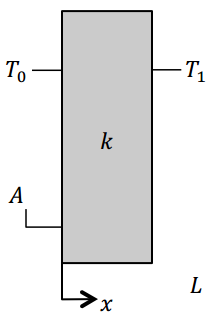
\includegraphics[scale=0.6]{figures/ch2/1}
    \caption{Model of example \ref{example:2:1}}
    \label{fig:2:1}
\end{figure}
\end{example}

\begin{solution}
~\\
For the plan wall, the heat resistance is
$$R=\frac{L}{kA}$$
So the heat rate 
$$
Q=\frac{\delta T}{R}=kA\frac{T_0-T_1}{L}=1000~W
$$

\begin{lstlisting}
Plot1=Plot[$T_0$ + x/L*($T_1-T_0$),{x, 0, L}]
\end{lstlisting}
The heat flux$$q=\frac{Q}{A}==1000~W/m^2$$
\begin{lstlisting}
R=L/(k*A); (*Resistance*)
$T_0$=50; (*Temperature on the other side of the wall)
$T_1$=30;
Q=($T_0$-$T_1$)/R; (*Watt5s*)
FLUX=Q/A;
\end{lstlisting}
Based on Fourier’s Law, the heat rate
\begin{eqnarray*}
Q=-kA\frac{dT}{dx}\\
dT=-\frac{Q}{ka}dx
\end{eqnarray*}
~\\
Integral
$$\int dT=-\int \frac{Q}{ka} dx$$
In steady state,  is constant, so the heat distribution along the x direction is
$$T(x)=C_1x+C_2$$
As given, $T(0)=T_0=50~K, T(0.01)=T_1=30~K$, we can get
$$T(x)=\frac{T_1-T_0}{L}x+T_0=-2000x+50$$
And the sketch of  is shown as figure \ref{fig:2:2}.
\begin{lstlisting}
Plot2=ListPlot[{{0,50},{0.01,30}},
      PlotStyle->{AbsolutePointSize[8]},
      AxesLabel->{Distance (m),Temperature}]
\end{lstlisting}

\begin{figure}[h!]
  \centering
    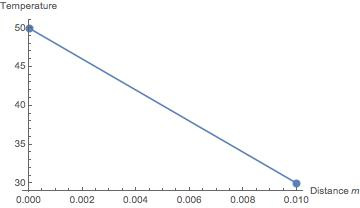
\includegraphics[scale=0.8]{figures/ch2/2}
    \caption{result}
    \label{fig:2:2}
\end{figure}
\end{solution}

\begin{example}
\label{example:2:2}
\textbf{Conical section} \textcolor{blue} {\emph{Refer to tutorial 
Prob\_ 7 copy.nb, and Ch. 3, P. 134.}}A diagram shows a conical section 
fabricated from pyroceram, $k=3.46W/m.K$. It is of circular cross section with 
the diameter $D=ax$, where $a=0.25$.The small end is at $x_1=50~mm$ and the large end at $x_2=250~mm$.
The end temperature are $T_1=400~K$ and $T_2=600~K$, while the lateral 
surface is well insulated.
\begin{enumerate}
\item Derive and expression for the temperature distribution $T(x)$,
assuming one-dimensional conditions. Sketch the temperature distribution.
\item Calculate the heat rate $Q$ through the cone.
\item If $a$ changes from 0.001 to 1, sketch change of $Q$.
\end{enumerate}
\begin{figure}[h]
  \centering
    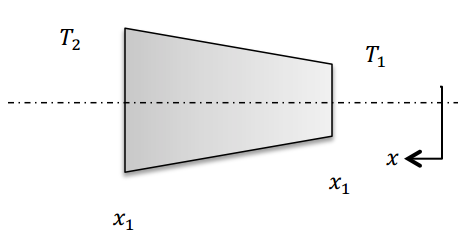
\includegraphics[scale=0.6]{figures/ch2/3}
    \caption{Model of example \ref{example:2:2}}
    \label{fig:2:3}
\end{figure}
\end{example}

\begin{solution}
~//
\begin{enumerate}
\item
Consider the heat conduction is under steady state, one-dimensional coordinate,
without internal heat generation, the heat transfer rate is a constant independent
of $x$. Use Fourier’s Law to determine the temperature distribution.
$$Q=-kA\frac{dT}{dx}$$
Where $A=\frac{\pi D^2}{4}=\frac{\pi a^2x^2}{4}$. Separating variables,
$$\frac{4Qdx}{\pi a^2x^2}=-kdT$$
Integrating from $x_1$ to any $x$ within the cone, and recalling that $Q$ and $k$
are constant, it follows that
$$\frac{4Q}{\pi a^2}\int_x^{x_1} dx/x^2=-k\int dT$$
Hence
$$\frac{4Q}{\pi a^2}\left(-\frac{1}{x}+\frac{1}{x_1}\right)=-k\left(T-T_1\right)$$
and
$$T(x)=T_1-\frac{4Q}{\pi a^2}\left(\frac{1}{x_1}-\frac{1}{x}\right)$$
Although $Q$ is a constant, it is as yet an unknown.
However, it may be determined by evaluating the above expression at
$x=x_2$, where $T(x_2)=T_2$. Hence
$$Q=\frac{\pi a^2k(T_1-T_2)}{4[(1/x_1)-(1/x_2)]}$$
and solving for Q
\begin{lstlisting}
Q =*a^2*k*(- )/(4((1/x1)-(1/x2))) (*  Watts  *)
\end{lstlisting}
Substituting for $Q$ into the expression for $T(x)$,
the temperature distribution becomes
$$T_2=T_1+(T_1-T_2)\left[\frac{(1/x)-(1/x_2)}{(1/x_1)-(1/x_2)}\right]$$
\begin{lstlisting}
Q =*a^2*k*(- )/(4((1/x1)-(1/x2))) (*  Watts  *)
\end{lstlisting}
From the result, temperature may be calculated as a function of $x$
and the distribution is as shown in figure \ref{fig:2:4}.
\begin{lstlisting}
Plot2 = Plot[T, {x, .05, .25}, PlotRange -> All, 
AxesLabel -> {Distance (m), Temperature }]
\end{lstlisting}
\begin{figure}[h!]
  \centering
    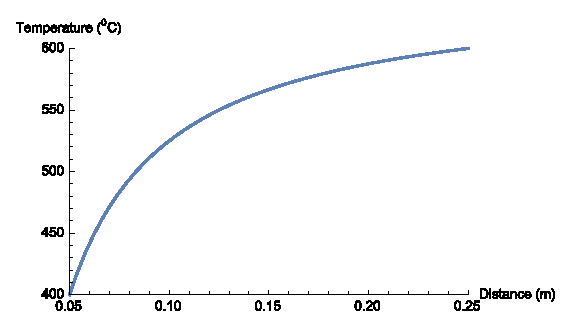
\includegraphics[scale=0.8]{figures/ch2/4}
    \caption{result of 1}
    \label{fig:2:4}
\end{figure}
\item
Substituting numerical values into the foregoing result for the heat 
transfer rate, it follows that
$$Q=\frac{\pi 0.25^2\times3.46~\text{W/m.K}\times(400-600)~K}{4(1/0.05~m - 1/0.25~m)}=-2.12W$$
\item
If $a$ changes from $0.001$ to $1$, as $Q$ has expression changes with $a$,
we can sketch $Q$’s changes with $a$ as shown in figure \ref{fig:2:5}.
\begin{figure}[h!]
  \centering
    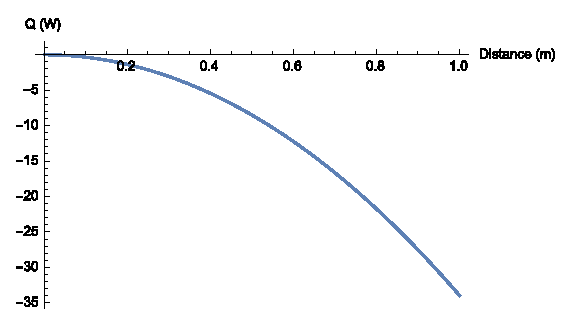
\includegraphics[scale=0.8]{figures/ch2/5}
    \caption{result of 3}
    \label{fig:2:5}
\end{figure}
\begin{lstlisting}
Qax =  *x^2*   k*(- )/(4 ((1/x1) - (1/x2)))
PlotQ = Plot[Qax, {x, .001, 1}, PlotRange -> All,    AxesLabel -> {"a", "Q" }]
\end{lstlisting}
\end{enumerate}
\end{solution}

\section{1-D steady state, constant	internal heat generation problems}
\begin{example}
\label{example:23}
\textcolor{blue} {\emph{Refer to tutorial HW\_1\_MMATICA.nb}}
A large thin slab of thickness $L=0.1~m$ is “setting.” Setting is an exothermic process 
that releases $\dot{q}=100W/m^3$. Here the slab heat conductivity is in steady state. 
Set the x-axis along with the wall thickness. At position $x=0m$, temperature is $T_0=37~K$,
at position $x=L$,$T_1=33~K$, thermal conductivity $k=0.4W/m.K$. What’s the
temperature distribution in along the length of the slab? 
\begin{figure}[h!]
  \centering
    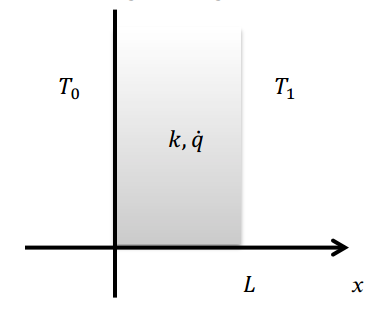
\includegraphics[scale=0.6]{figures/ch2/6}
    \caption{Model of example \ref{example:23}}
    \label{fig:2:6}
\end{figure}
\end{example}

\begin{solution}
~\\
Based on the heat diffusion equation 
$$\nabla^2 T+\frac{\dot{q}}{k}=\frac{1}{\propto}\frac{\partial T}{\partial t}$$
where
$$\nabla^2 T \equiv \frac{\partial^2 T}{\partial x^2}+
\frac{\partial^2 T}{\partial y^2}+
\frac{\partial^2 T}{\partial z^2}$$
In this problem, the large thin slab could be considered as a one-dimensional problem 
with only $x$ dimension, and consider the slab is in steady state with no change with $t$,
so the one-dimensional heat diffusion equation for the slab could be write as
$$\frac{d^2 T}{d x^2}=-\frac{\dot{q}}{k}$$
\begin{lstlisting}
solution1 = NDSolve[{T''[x] + /k == 0, T[0] == ,  T[0.1] == }, T, {x, 0, 0.1}];
\end{lstlisting}
Integration twice
$$T(x)=-\frac{\dot{q}}{2k}x^2+C_1x+C_2$$
By evaluating $T(0)=T_0$, and $T(L)=T_1$, hence
$$T(x)=-\frac{\dot{q}}{2k}x^2+ \left(\frac{T_1-T_0}{L}+\frac{\dot{q}L}{2k}\right)x+T_0$$
From the result, temperature distribution could be expressed as a quadratic curve as shown in
figure \ref{fig:2:7}.
\begin{lstlisting}
PS1 = Plot[Evaluate[T[x] /. First[solution1]], {x, 0, 0.1},    PlotRange -> All]
\end{lstlisting}
\begin{figure}[h!]
  \centering
    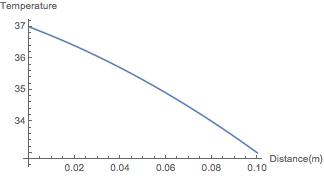
\includegraphics[scale=0.8]{figures/ch2/7}
    \caption{result}
    \label{fig:2:7}
\end{figure}
\end{solution}

\begin{example}
\label{example:24}
\textcolor{blue} {\emph{Refer to tutorial HW\_1\_MMATICA.nb, and Ch. 3, P. 134.}}
A steady state long tube generating thermal energy at a uniform volumetric rate
$\dot{q}=1000W/m^3$, the thermal conductivity $k=0.4$W/m.K.
At radius $r_1=0.1368m$, temperature $T_0=37~K$, at position $r_2=0.1768m$
, temperature $T_1=33~K$, the two end of the rod are well insulated.
What is the temperature distribution along the radius of the tube?
\begin{figure}[ht!]
  \centering
    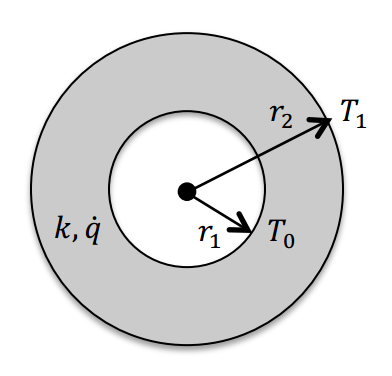
\includegraphics[scale=0.6]{figures/ch2/8}
    \caption{Model of example \ref{example:24}}
    \label{fig:2:8}
\end{figure}
\end{example}

\begin{solution}
~
The heat diffusion equation for cylindrical system is 
$$ 
\frac{1}{r}\frac{\partial}{r}(kr\frac{\partial T}{\partial r})+
\frac{1}{r^2}\frac{\partial}{\phi}(k\frac{\partial T}{\partial \phi})+
\frac{\partial}{z}(k\frac{\partial T}{\partial z})+
\dot{q} =
\rho c_p\frac{\partial T}{\partial t}
$$
In this problem, consider the heat distribution change only on $r$ direction,
and since the tube is in steady state, the temperature distribution would not
change with time $t$. The heat distribution equation could be written as
$$\frac{1}{r}\frac{\partial}{r}(kr\frac{\partial T}{\partial r})+\dot{q}=0$$
Integration twice
$$T(r)=-\frac{\dot{q}}{4k}r^2+C_1Inr+C_2$$
Substituting $T(r_1)=T_0$, $T(r_2)=T_1$, hence
$$
T(r)=-\frac{\dot{q}}{4k}r^2 +\left[\frac{T_1-T_0+(\dot{q}/4k)\cdot r_2^2}{In(r_2/r_1)} \right]\cdot Inr +
\frac{T_0Inr_2-T_1Inr_1-(\dot{q}/4k)\cdot r_2^2}{In(r_2/r_1)}
$$
~\\
By evaluating $r_1=0.1368~m, T_0=37~K, r_2=0.1768~m \text{and} T_1=33~K$,
sketch the $T(r)$ as shown in figure \ref{fig:2:9}
\begin{figure}[h!]
  \centering
    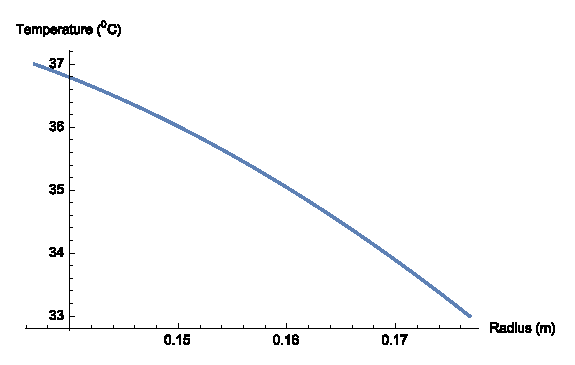
\includegraphics[scale=0.6]{figures/ch2/9}
    \caption{result}
    \label{fig:2:9}
\end{figure}
\end{solution}

\section{1-D steady state, variate internal	heat generation	problems}
\begin{example}
\textcolor{blue} {\emph{Refer to tutorial HW\_1\_MMATICA.nb, Ch. 3, P. 178.}}
Consider the slab in the example \ref{example:23} and the tube in example
\ref{example:24} are human tissues, the blood perfusion heat that varies with the internal temperature. The blood mass rate per volumetric tissue is $m_b=100kg/s$, specific heat capacity of blood $50J/kg.K$, initial temperature of the blood is 
$T_a=37K$. Except the internal heat generation, other parameters are the same. 
Sketch the temperature distribution in the slab and the tube.
\end{example}

\begin{solution}
~
\begin{enumerate}
\item
Based on the bioheat equation, the volumetric heat rate diffused by the blood into the tissue is 
$$q_b=m_b c_b(T_a-T)$$
set$$\theta = T-T_a$$
hence based on the 1-D steady state heat diffusion equation in Cartesian coordinate
where $\gamma^2=m_b c_b/k$, the boundary condition $T(0)=T_0$ and  $T(L)=T_1$,
the solution for $\theta$ is as below
$$\frac{\theta}{\theta_0}=\frac{\sinh\gamma x+\sinh\gamma(L-x)}{\sinh\gamma L}$$
sketch of $\theta(x)$ is as below.
\begin{figure}[h!]
  \centering
    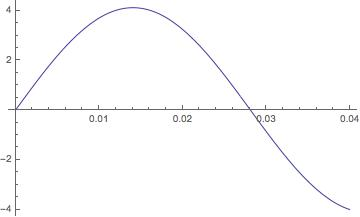
\includegraphics[scale=0.6]{figures/ch2/10}
    \caption{result of 1}
    \label{fig:2:10}
\end{figure}
\item
For the tube, the cylindrical equation is
$$\frac{d^2 \theta}{dr^2} + \frac{1}{r}\frac{d\theta}{dr}-\gamma^2\theta=0$$
Solve this equation and get the sketch of $\theta(r)$
\begin{figure}[h!]
  \centering
    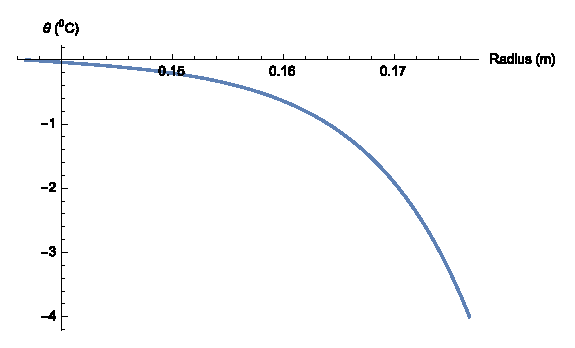
\includegraphics[scale=0.8]{figures/ch2/11}
    \caption{result of 2}
    \label{fig:2:11}
\end{figure}
\end{enumerate}
\end{solution}

\section{Fin problems}
\begin{example}
\label{example:2:fin}
\textbf{Constant k and A}. 
\textcolor{blue} {\emph{Refer to tutorial 3.  Fin Solutions 2.nb, Ch. 3, P. 157}}
A rectangular fin with uniform cross-sectional area has constant heat conductivity
$k=3W/m.K$, width is $W=0.01m$, Thickness is $L=1m$. At start position $x_1=0m$, temperature is $T_1=30^\circ C$. The surface of the fin is exposed to ambient air at $10K$ with a convection heat transfer coefficient $h=10W/m^2K$.
Plot the temperature distribution in the fin under below conditions. (Shown in figure \ref{fig:2:12})
\begin{enumerate}
\item Prescribed tip temperature: at the end position $x_2=0.04m, T_2=40^\circ C$
\item Adiabatic tip condition.
\item Infinite tip condition.
\end{enumerate}
\begin{figure}[h!]
  \centering
    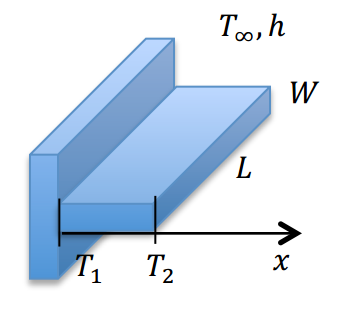
\includegraphics[scale=0.7]{figures/ch2/12}
    \caption{Model of example \ref{example:2:fin}}
    \label{fig:2:12}
\end{figure}
\end{example}

\begin{solution}
~
\begin{enumerate}
\item
The fin energy balance equation
$$
\frac{d^2 T}{dx^2} + 
\left(\frac{1}{A_c}\frac{dA_c}{x}\right)\frac{dT}{dx}-
\left(\frac{1}{A_c}\frac{h}{k}\frac{dA_s}{x}\right)(T-T_\infty)=0
$$
For the proscribed fin problem with constant cross section area $A_c=WL$ , 
and surface area, we have $dA_c/dx=0$, $dAs/dx=p$. Hence
$$
\frac{d^2 T}{dx^2}-
\frac{hp}{kA_c}(T-T_\infty)=0
$$
To simplify the form of this equation, we transform the dependent variable by 
defining an excess temperature $\theta$ as
$$\theta(x) \equiv T(X)-T_\infty$$
Where since $T_\infty$ is constant, $d\theta/dx=dT/dx$. Then we obtain
$$\frac{d^2 T}{dx^2}-m^2\theta=0$$
Where
$$m^2 \ equiv \frac{hp}{kA_c}$$
With prescribed boundary condition
$$\theta(0)=T_1-T_\infty \equiv \theta_1$$
$$\theta(0.04)=T_2-T_\infty \equiv \theta_2$$
Then for prescribed condition the fin temperature distribution is
$$
\frac{\theta}{\theta_1}=
\frac{(\theta/\theta_1)\sinh mx+\sinh m(L-x)}{\sinh mL}
$$
\begin{figure}[h!]
  \centering
    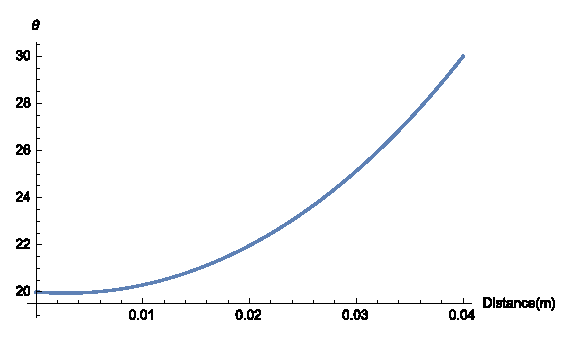
\includegraphics[scale=0.8]{figures/ch2/13}
    \caption{result of 1}
    \label{fig:2:13}
\end{figure}
\item
For adiabatic tip condition, the heat convection rate at the tip is considered negligible
$$hA_c\theta(L)=-k\frac{d\theta}{dx}|_{x=L}=0$$
And
$$\frac{d\theta}{dx}|_{x=L}=0$$
Then the heat distribution equation of adiabatic tip condition could be written as
$$\frac{\theta}{\theta_1}=
\frac{\cosh m(L-x)}{\cosh mL}
$$
The temperature distribution along x direction is shown below
\begin{figure}[h!]
  \centering
    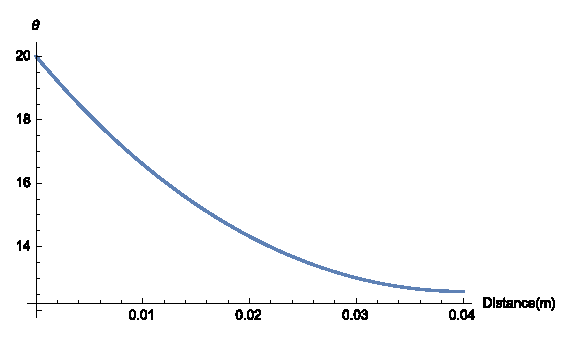
\includegraphics[scale=0.8]{figures/ch2/14}
    \caption{result of 2}
    \label{fig:2:14}
\end{figure}
\item
For an infinite fin the tip is  $x\to\infty$, and the boundary condition at the tip is 
$$\theta(0.04)=0$$
And the temperature distribution is 
$$\frac{\theta}{\theta_1}=e^{-mx}$$
Sketch the temperature distribution
\begin{figure}[h!]
  \centering
    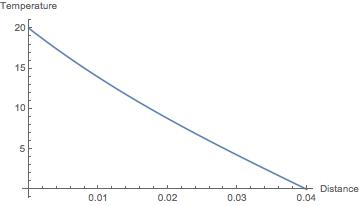
\includegraphics[scale=0.8]{figures/ch2/15}
    \caption{result of 3}
    \label{fig:2:15}
\end{figure}

\end{enumerate}
\end{solution}


\begin{example}
\label{example:2:Noncons}
\textbf{Non constant cross sectional problem}
\textcolor{blue} {\emph{Refer to tutorial 3.  Fin Solutions 2.nb, Ch. 3, P. 167.}}
A dylindrical fin with has constant heat conductivity  $k=3W/m.K$, width is
$W=0.01m$. At start position $r_1=0.0001m$, temperature is $T_1=30K$. Radius at
the end of fin is $r_2=0.04m$. The surface of the fin is exposed to ambient air at
$10K$ with a convection heat transfer coefficient $h=10W/m^2K$.
Plot the temperature distribution in the fin under below conditions. (Shown in figure \ref{fig:2:16})

\begin{enumerate}
\item Prescribed tip condition, at $r_2=0.04m$, temperature $T_2=40~K$
\item Infinite tip condition.
\end{enumerate}
\begin{figure}[h!]
  \centering
    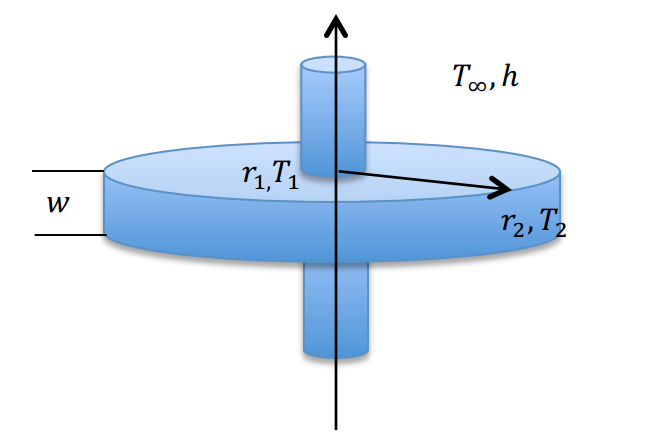
\includegraphics[scale=0.4]{figures/ch2/16}
    \caption{Model of example \ref{example:2:Noncons}}
    \label{fig:2:16}
\end{figure}
\end{example}

\begin{solution}
~\\
\begin{enumerate}
\item For a cylindrical fin, the cross section area $A_c=2\pi rw$,
surface area $A_s=2\pi(r^2-r_1^2)$, replace $x$ by $r$ in
$$
\frac{d^2 T}{dx^2} + 
\left(\frac{1}{A_c}\frac{dA_c}{x}\right)\frac{dT}{dx}-
\left(\frac{1}{A_c}\frac{h}{k}\frac{dA_s}{x}\right)(T-T_\infty)=0
$$
and get
$$
\frac{d^2 T}{dr^2}+
\frac{1}{r}\frac{dT}{dr}-
\frac{2h}{kw}(T-T_\infty)=0
$$
with $m^2 \equiv 2h/kw \text{and} \theta=T-T_\infty$
$$
\frac{d^2 \theta}{dr^2}+
\frac{1}{r}\frac{d\theta}{dr}-
m^2\theta=0
$$
For proscribed tip problem, boundary condition is 
$$\theta(0)=T_1-T_\infty \equiv \theta_1$$
$$\theta(0.04)=T_2-T_\infty \equiv \theta_2$$

Solve this two step differential equation with Mathematica and get the sketch of temperature distribution as below
\begin{figure}[h!]
  \centering
    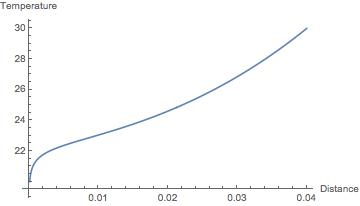
\includegraphics[scale=0.8]{figures/ch2/17}
    \caption{result of 1}
    \label{fig:2:17}
\end{figure}
\item For infinite boundary condition
$$\theta(r_2)=\theta(0.04)=0$$
Solve this two step differential equation with Mathematica and get the sketch of temperature distribution as below
\begin{figure}[h!]
  \centering
    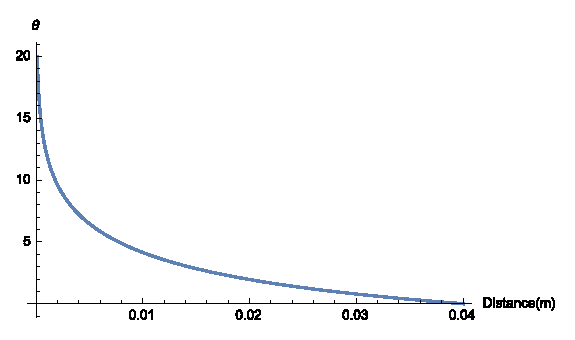
\includegraphics[scale=0.8]{figures/ch2/18}
    \caption{result of 2}
    \label{fig:2:18}
\end{figure}
\end{enumerate}
\end{solution}













